\chapter{Problem Analysis}

% Detailed Analysis of the Problem: Go deeper into the specific challenges and problems within motion tracking, especially those that AI could address.

% Theoretical and Practical Implications: Discuss both theoretical and real-world implications of improving AI-based motion tracking.

\section{Overview}
The convergence of artificial intelligence (AI) and motion tracking technologies represents a pivotal moment for innovation across various fields, including healthcare, sports analytics, robotics, and entertainment. Despite their potential, the integration of these two domains faces numerous challenges, which hinder accessibility and scalability. This chapter delves into the problem space by analyzing the current limitations, defining the research objectives, and establishing the scope and significance of the study.

By addressing these challenges, the proposed research seeks to contribute to the democratization of AI-driven motion tracking systems, fostering widespread adoption and innovation.

\section{Background and Context}
Motion tracking, enabled by devices such as inertial measurement units (IMUs), cameras, and wearable sensors, is a critical enabler of applications that require precise understanding of movement. Recent advancements have led to the development of systems capable of tracking complex motions in real-time. Examples include:

\begin{itemize}
    \item Healthcare: Monitoring rehabilitation progress and detecting fall risks.
    \item Sports: Analyzing athletes’ performance to optimize training.
    \item Entertainment: Enabling realistic motion capture in animation and gaming.
\end{itemize}

However, integrating motion tracking with AI introduces complexities that stem from technological and practical barriers. Although platforms such as Edge Impulse and Google MediaPipe offer powerful capabilities, their utility is often constrained by:

\begin{itemize}
    \item The need for technical expertise to design, train, and deploy AI models.
    \item Hardware limitations that restrict real-time processing on edge devices.
    \item A lack of standardization across datasets, making it challenging to generalize AI models.
\end{itemize}

% Motion Tracking Ecosystem Diagram
% A diagram illustrating the components of a typical motion tracking system:
% Sensors (e.g., IMU, camera).
% AI frameworks (e.g., Edge Impulse, MediaPipe).
% Processing (e.g., edge device, cloud).
% Applications (e.g., healthcare, sports).
% Purpose: Highlights the complexity of integrating motion tracking and AI.
\begin{figure}
    \centering
    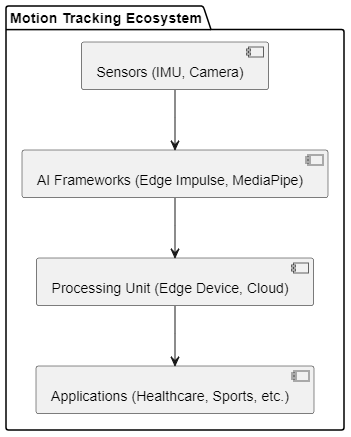
\includegraphics[width=0.5\linewidth]{images//chapter_4/motion_tracking_ecosystem_diagram.png}
    \caption{Motion Tracking Ecosystem Diagram}
    \label{fig:enter-label}
\end{figure}

Without a user-friendly framework, these challenges remain significant hurdles for researchers, developers, and end-users alike.

\section{Problem Definition}
Despite the potential of AI to revolutionize motion tracking, several key issues persist:

\begin{enumerate}
    \item Complexity for Non-Experts:
    The creation and deployment of AI models for motion tracking often require expertise in multiple domains, including machine learning, sensor fusion, and hardware optimization.
    
    For instance, researchers must preprocess raw sensor data, extract meaningful features, and train models, all of which demand specialized knowledge.

    \item Scalability and Adaptability:
    Many existing solutions are tailored for specific use cases, such as clinical gait analysis or virtual reality applications, making them unsuitable for broader adoption.
    
    Lack of modularity in frameworks hinders adaptability to diverse scenarios.

    \item Hardware Limitations:
    Resource-constrained devices like wearables have limited computational power, memory, and battery life, making it difficult to implement and run complex AI models.

    \item Data Challenges:
    Motion tracking systems depend heavily on high-quality data, yet variability in sensor performance, environmental factors, and user movements often lead to noisy or incomplete datasets.

    \item Cost Barriers:
    Advanced motion tracking systems, such as optical motion capture setups, are prohibitively expensive, restricting their use to high-budget projects or well-funded institutions.
\end{enumerate}

\pagebreak

\begin{table}
    \centering
    \label{tab:tab_4}
    \caption{Problem Summary Table}
    \begin{tabular}{| >{\centering\arraybackslash}m{3cm} | >{\centering\arraybackslash}m{5cm} | >{\centering\arraybackslash}m{4cm} |}
        \toprule
         \textbf{Challenge} &  \textbf{Description}& \textbf{Impact}\\
         \midrule
         Complexity &  Requires expertise in AI, sensor fusion, and hardware optimization.& Limited accessibility for non-experts.\\
         \hline
         Scalability &  Frameworks often tailored to specific use cases.& Difficult to generalize or adapt.\\
         \hline
         Hardware Limitations &  Limited computational power on edge devices.& Performance bottlenecks.\\
         \hline
         Data Challenges &  Variability and noise in motion data.& Reduces model accuracy.\\
         \hline
         Cost Barriers &  Advanced systems are expensive.& Limits adoption in low-budget settings.\\
         \bottomrule
    \end{tabular}
\end{table}

Addressing these challenges necessitates a framework that simplifies AI model generation while being resource-efficient, adaptable, and accessible.

\section{Objectives of the Research}
This research aims to overcome the identified challenges by focusing on the following objectives:

\begin{enumerate}
    \item Framework Development:
    Develop a user-friendly framework that facilitates the creation and deployment of AI models for motion tracking. The framework should abstract the technical complexities to enable usage by non-experts.
 
    \item Compatibility with Edge Devices:
    Design the framework to be compatible with resource-constrained devices, such as the Seeed XIAO nRF52840 Sense, ensuring real-time processing with minimal energy consumption.

    \item Data Preprocessing and Model Optimization:
    Incorporate automated methods for data preprocessing, feature extraction, and model optimization to improve accuracy and robustness.

    \item Evaluation and Comparison:
    Provide tools for evaluating and comparing AI models across various motion tracking applications, enabling users to choose the most suitable model for their needs.

    \item Scalability:
    Ensure the framework supports diverse applications, from healthcare monitoring to sports analytics, while being modular and adaptable.
\end{enumerate}

% Framework Goals Flowchart
% A flowchart depicting the objectives of the framework:
% Data Preprocessing → 2. Model Generation → 3. Optimization → 4. Evaluation.
% Purpose: Illustrates the logical flow of how the framework will address the challenges.
\begin{figure}
    \centering
    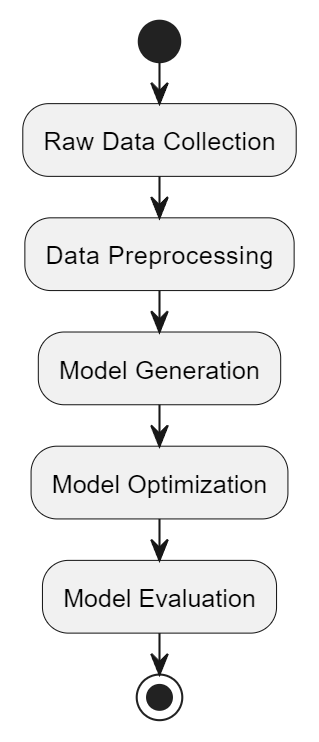
\includegraphics[width=0.25\linewidth]{images//chapter_4/framework_goal_flowchart.png}
    \caption{Framework Goals Flowchart}
    \label{fig:enter-label}
\end{figure}

\section{Scope of the Research}
The research is focused on developing a framework that bridges the gap between motion tracking systems and AI. Key aspects of the scope include:

\begin{itemize}
    \item Primary Focus:
    The study will center on designing and implementing an AI model generation framework tailored for motion tracking applications.

    \item Exclusions:
    While the research explores motion data processing and AI integration, it will not delve into unrelated AI domains such as natural language processing or image-based tracking.

    \item Hardware Agnosticism with Specific Examples:
    Although the proposed framework will be evaluated using specific hardware like the Seeed XIAO nRF52840 Sense, the design principles will be adaptable to other devices.
\end{itemize}

% Scope Illustration
% A Venn diagram showing:
% The intersection between motion tracking, AI frameworks, and edge computing.
% Excluded areas (e.g., image-based tracking, natural language processing).


This scoped approach ensures the research remains focused and achievable within the given timeframe.

\section{Significance of the Study}
The proposed framework addresses several key gaps in current motion tracking and AI systems:

\begin{enumerate}
    \item For Researchers:
        Provides a structured approach to model development, reducing time and effort spent on repetitive tasks.
        Promotes innovation by enabling experiments with different AI models and techniques.

    \item For Developers:
        Reduces the technical barriers to entry, fostering broader adoption of AI in motion tracking applications.
    
    \item For End Users:
        Enables cost-effective solutions that can be deployed in real-world scenarios, such as wearable health monitoring or virtual reality gaming.
\end{enumerate}

\pagebreak

\begin{table}
    \centering
    \caption{Research Question Mapping }
    \label{tab:tab_5}
    \begin{tabular}{| p{5cm} | p{4cm} | p{4cm} |}
        \toprule
        \textbf{Research Question} & \textbf{Related Objective} & \textbf{Challenge Addressed}\\
        \hline
        How can the framework abstract complexities?&  Develop a user-friendly framework.& Complexity, Scalability.\\
        \hline
        What preprocessing techniques are most effective?&  Automate preprocessing and feature extraction.& Data Challenges.\\
        \hline
        How can the framework support edge devices?&  Optimize for resource-constrained devices.& Hardware Limitations.\\
        \hline
        What metrics best evaluate AI motion tracking systems?&  Provide robust evaluation methods.& Scalability, Usability.\\
        \bottomrule
    \end{tabular}
\end{table}

By simplifying AI model generation and deployment, the framework could accelerate the adoption of AI-powered motion tracking systems, benefiting multiple industries and stakeholders.

\section{Research Questions}
The following research questions guide the study:

\begin{enumerate}
    \item How can the proposed framework abstract the complexities of AI model generation for motion tracking applications?
    \item What preprocessing and optimization techniques are most effective for motion data?
    \item How can the framework be adapted to resource-constrained devices without compromising performance?
    \item What evaluation metrics best reflect the performance of AI models in motion tracking systems?
\end{enumerate}

\section{Summary}
This chapter provided a comprehensive analysis of the research problem, defined the objectives, and outlined the scope and significance of the study. By addressing the challenges identified, the research aims to make AI-powered motion tracking systems more accessible, scalable, and effective. The next chapter will detail the research methodology, laying the groundwork for achieving these objectives.
